\documentclass{lug}

\usepackage{csquotes}
\MakeOuterQuote{"}
\usepackage{listings}

\title{Git}
\author{Sumner Evans}

\begin{document}

\begin{frame}
    \frametitle{What is Git?}

    \begin{itemize}[<+->]
        \item Git is a system which tracks changes made to a code base.
        \item Git was created by Linus Torvalds to help facilitate Linux kernel development.
        \item Linus's motto when he built Git was to take Concurrent Version System (CVS) as an
            example of what \textit{not} to do and if in doubt, make the opposite decision.
            \footnotemark
    \end{itemize}

    \uncover<3>{\footnotetext[1]{https://en.wikipedia.org/wiki/Git}}
\end{frame}

\begin{frame}
    \frametitle{Why use Version Control? I}

    Example Scenario:

    \begin{enumerate}[<+->]
        \item You start a project called "my-proj" and write a ton of code.
        \item You finally get it to (kinda) work.
        \item You decide to make a copy of "my-proj" for backup purposes.
        \item You continue development on "my-proj" but then screw something up really bad.
        \item You decide to revert back to your copy.
        \item Then you realize your copy doesn't have a bug fix that you actually wanted.
        \item You then proceed to manually compare the files in the backup to those in your new code
            and figure out what you still want to have.
    \end{enumerate}

    \uncover<8>{This is terrible.}
\end{frame}

\begin{frame}
    \frametitle{Why use Version Control? II}

    Another Scenario:

    \begin{enumerate}[<+->]
        \item You start working on a project with a partner.
        \item You write a bunch of code.
        \item You email the code in a .zip file, then go home for the weekend.
        \item You and your partner had decided to work on two separate tasks over the weekend so you
            make some changes to the code and your partner makes some changes to the code.
        \item You come together and start copying files. Then you realize you both modified
            \texttt{main()}.
        \item You then manually determine what changed in both files and reconcile them.
    \end{enumerate}

    \uncover<7>{This is awful.}
\end{frame}

\begin{frame}
    \frametitle{Why use Version Control? III}

    How Version Control Systems (VCS) solve this:

    \begin{itemize}[<+->]
        \item VCS keeps track of \textit{revisions}, changes in the code in entities called
            \textit{changesets} or \textit{commits}.
        \item Most VCS allow version merging. That means multiple people can be working on the same
            file and resolve discrepancies later. Git is very elegant in handling merge conflicts
            such as this.
    \end{itemize}
\end{frame}

\begin{frame}
    \frametitle{Why use Git?}

    Git is a VCS so it solves all of the issues I've described. So why use Git over some other
    VCS?\footnotemark

    \begin{itemize}[<+->]
        \item It's a \textit{distributed} VCS. That means that you have a full copy of the code and
            every change ever made by anyone to that code on your local machine. A beneficial side
            effect of this is that you can work offline.
        \item It's faster.
        \item Git rarely fully deletes anything, this is good because you can undo most actions.
        \item Everyone else is using it.
    \end{itemize}

    \footnotetext[2]{List inspired by
    \url{https://www.git-tower.com/blog/8-reasons-for-switching-to-git}}
\end{frame}

\begin{frame}
    \frametitle{How to Get Git}

    Git is awesome! How do I get it? \textbf{Good news: Git is cross platform.}

    \begin{itemize}
        \item \textbf{Linux:} Install the \texttt{git} package using your distribution's package
            manager
        \item \textbf{OS X:} I recommend using Homebrew: \texttt{brew install git}
            (\url{http://brew.sh/})
        \item \textbf{Windows:} Download the installer from \url{https://git-scm.com/}
    \end{itemize}

    If you need a GUI, check out SourceTree on macOS and Windows. If you need a GUI on Linux, you
    are doing Linux wrong.\\

    You should also setup SSH which is extremely easy, but I will not cover that here as this is a
    talk about Git not SSH.
\end{frame}

\begin{frame}
    \frametitle{Hot to use Git (locally)}

    \begin{itemize}
        \item Initialize (\texttt{git init}): Initializes a Git \textit{repository} on your local
            machine.
        \item Add (\texttt{git add}): Marks files to include in the next \textit{commit}, an entity
            which stores the state of the repository at a given time.
        \item Commit (\texttt{git commit}): Creates a commit.
        \item Log (\texttt{git log}): Shows the history of your repository.
        \item Diff (\texttt{git diff [file]}): Determines the difference between the file's current
            state and its state at the last commit.
        \item Git ignore (modify the \texttt{.gitignore} file): Any file that matches one of the
            patterns in \texttt{.gitignore} will not be tracked by Git.
    \end{itemize}
\end{frame}

\begin{frame}
    \frametitle{How to use Git with a remote}

    \begin{itemize}
        \item Add Remote (\texttt{git remote add}): Adds a remote to an existing local repository.
        \item Push (\texttt{git push -u origin master}): Pushes all changes on the given branch
            to the remote.
        \item Clone (\texttt{git clone}): Retrieves the entire repository to the location.
        \item Fetch (\texttt{git fetch}): Retrieves changes from the remote.
        \item Merge (\texttt{git merge}): Merges a branch into another branch. (More on branches
            later, but in this case, we are merging the \texttt{origin/master} into our local
            \texttt{master} branch.)
        \item Pull (\texttt{git pull}): Retrieves any new changes from the remote and merges them
            with your local changes.
    \end{itemize}
\end{frame}

\begin{frame}
    \frametitle{Merging Changes I}

    What happens if multiple developers make changes to the same file? This will cause \textit{merge
    conflicts}.\\

    There are plenty of tools which you can use to \textit{resolve} such conflicts. None of them are
    that good because merge conflicts are just terrible in general.\\

    Play around with a bunch of them and see which one you like best. Here are a few to get you
    started: \texttt{Meld}, \texttt{KDiff3}, and \texttt{vimdiff}.\\
\end{frame}

\begin{frame}
    \frametitle{Merging Changes II}

    Invoking the \textit{mergetool}: use \texttt{git mergetool}.\\

    For each \textit{conflict}, you can choose to take their version, your version, a combination of
    the two or neither.\\

    Most UIs will give you three panes: one for the \textit{remote} version of the file, one for the
    \textit{local} version of the file and one for the merged version of the file.

\end{frame}

\begin{frame}
    \frametitle{Branches I}

    Branches allow you to separate develop a given functionality without affecting the original code
    base.\\

    For example, if you have an established product and you want to add a feature but you are
    uncertain about its viability, you can create a branch and build a prototype on that branch. If
    it fails, you can delete the branch and never see it again or if it works, you can
    \textit{merge} the branch back into \texttt{master}.
\end{frame}

\begin{frame}
    \frametitle{Branches\footnotemark II}
    Branches can be thought of as \textit{bookmarks} pointing to a specific changeset.

    \begin{center}
        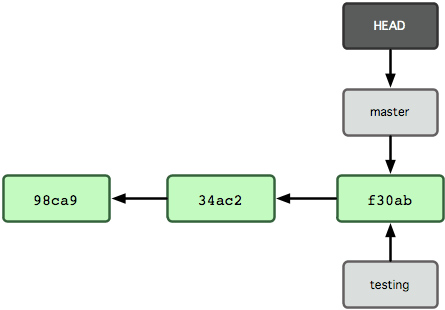
\includegraphics[width=60mm]{graphics/branching1.png}
    \end{center}

    \textit{Note, \texttt{HEAD} is pointer to the current branch.}

    \footnotetext[3]{Info in the rest of the \textit{Branches} section is mainly from
    \url{https://git-scm.com/book/en/v1/Git-Branching-What-a-Branch-Is}}
\end{frame}

\begin{frame}
    \frametitle{Branches III}
    To switch branches, use \texttt{git checkout [branch]}. This moves \texttt{HEAD} to point to
    your new branch.

    \begin{center}
        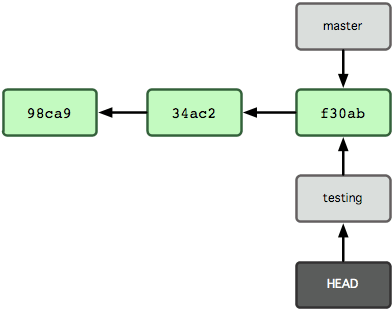
\includegraphics[width=65mm]{graphics/branching2.png}
    \end{center}
\end{frame}

\begin{frame}
    \frametitle{Branches IV}
    If you commit something to your new branch, the branch pointer moves to the new commit. The
    pointer to \texttt{master} will not move.

    \begin{center}
        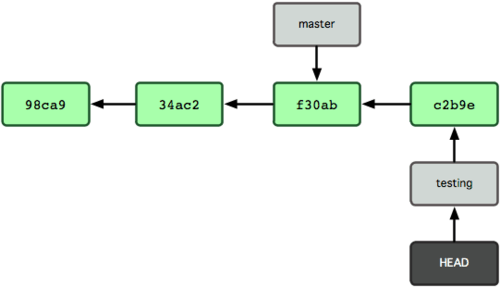
\includegraphics[width=65mm]{graphics/branching3.png}
    \end{center}
\end{frame}

\begin{frame}
    \frametitle{Branches V}
    Of course, you can always switch back to \texttt{master} using \texttt{git checkout master}.

    \begin{center}
        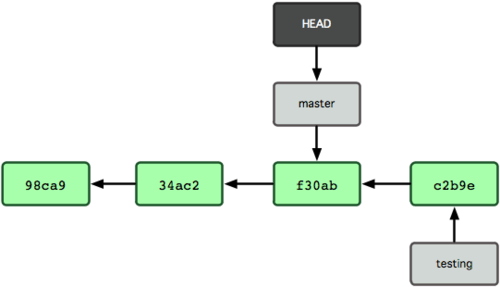
\includegraphics[width=65mm]{graphics/branching4.png}
    \end{center}
\end{frame}

\begin{frame}
    \frametitle{Branches VI}
    If you make a commit on the master branch, the \texttt{master} pointer moves to that new commit.
    At this point, the branch histories have diverged.

    \begin{center}
        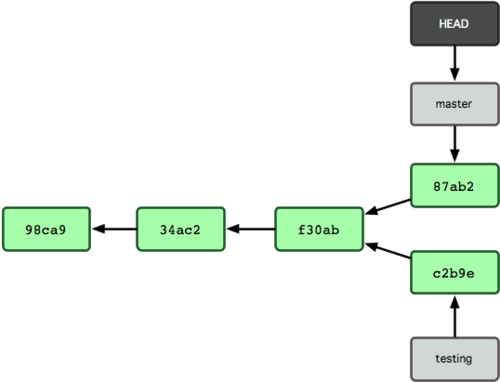
\includegraphics[width=65mm]{graphics/branching5.png}
    \end{center}
\end{frame}

\begin{frame}
    \frametitle{Branches VII: How to actually do it}

    \begin{itemize}
        \item \textbf{Create a Branch:} \texttt{git branch [branch\_name]}
        \item \textbf{Switch to a branch:} \texttt{git checkout [branch\_name]}
        \item \textbf{Create a new branch and switch to it:}\\ \texttt{git checkout -b [branch\_name]}
        \item \textbf{List branches:} \texttt{git branch}
        \item \textbf{Push branch to remote:} \texttt{git push -u [remote\_name] [branch\_name]}
    \end{itemize}
\end{frame}

\begin{frame}
    \frametitle{Merging Changes: Branch Edition}
    If you want changes from a different branch in your current branch, you can use \texttt{git
    merge [other branch]}.\\

    When you merge changes from another branch, one of two things will happen\footnotemark:

    \begin{enumerate}
        \item Your branch will be fast-forwarded to the other branch.\\
            This means that there are no changes in your current branch that are not in the other
            branch.
        \item A merge commit will be created and your branch pointer will be updated to point to
            this commit.\\
            This happens when there are changes in the current branch that are not in the other
            branch.
    \end{enumerate}

    \footnotetext[4]{These are the only ones I can thing of off the top of my head. You can force
    either of these functionalities with their respective command line options.}
\end{frame}

\begin{frame}
    \frametitle{Branch and Development Workflow}

    Branches are extremely scalable so you can ignore them, or use them for everything, it's your
    choice.\\

    One common methodology used by Agile companies is to use \texttt{Git Flow}. This has a system
    whereby new branches are created for every bugfix, new feature, release, and hotfix. If you want
    to learn more about it, look at this website:
    \url{http://nvie.com/posts/a-successful-git-branching-model/}
\end{frame}

\begin{frame}
    \frametitle{Cool Resources/Tips}

    \begin{itemize}
        \item \texttt{gitignore.io}: Generates a \texttt{.gitignore} file for a given project type,
            OS, and IDE.
        \item \texttt{git reset --hard HEAD}: Undoes all changes since the last commit.
            % TODO: More cool resources
        \item \texttt{git diff HEAD:file1 file2}: Shows the difference between \texttt{file1} and
            \texttt{file2}.
    \end{itemize}
\end{frame}

% Stuff that someone wants (at least I'm guessing that was his response)
%       Rebasing
%       Rewriting History
%       Creating git instances on remote servers (that aren't github or bitbucket)
%       What can git do that I've never even heard about?

% Lifesavers
%       Move commit to another branch

% Advanced Git topics to add:
%       gitignore
%       branching
%               flow
%       fetch vs push
%       saving your butt
%       stashing
%       other stuff
%       add--interactive
%       alias
%       collapse commit (TODO: Look up term)
%       revert
%       reset

\end{document}
